\documentclass[12pt]{article}
%Gummi|065|=)
\usepackage{amsmath, amsfonts, amssymb}
\usepackage[margin=0.5in]{geometry}
\usepackage{xcolor}
\usepackage{graphicx}
\newcommand{\off}[1]{}
\DeclareMathSizes{20}{30}{21}{18}



\newcommand{\myhrule}{}

\usepackage{tikz}

\title{\textbf{ An Inversion Problem }}
\author{John D Mangual}
\date{}
\begin{document}

\fontfamily{qag}\selectfont \fontsize{24}{30}\selectfont

\maketitle

\noindent I ask around for a solution to an inversion problem.  Everyone could show me \textbf{how} to solve it but nobody wanted put the solution\footnote{I didn't ask ``how would you solve it" -- I was asking for an explicity answer, with a center and a radius.  Nobody wanted to.  If you do it neatly takes about a page (or less).  If you don't know algebra it takes 10 pages and you get nowhere.  This was a skill in textbook in 19th century -- and in fact all of my resources come from that time period.} \\ 
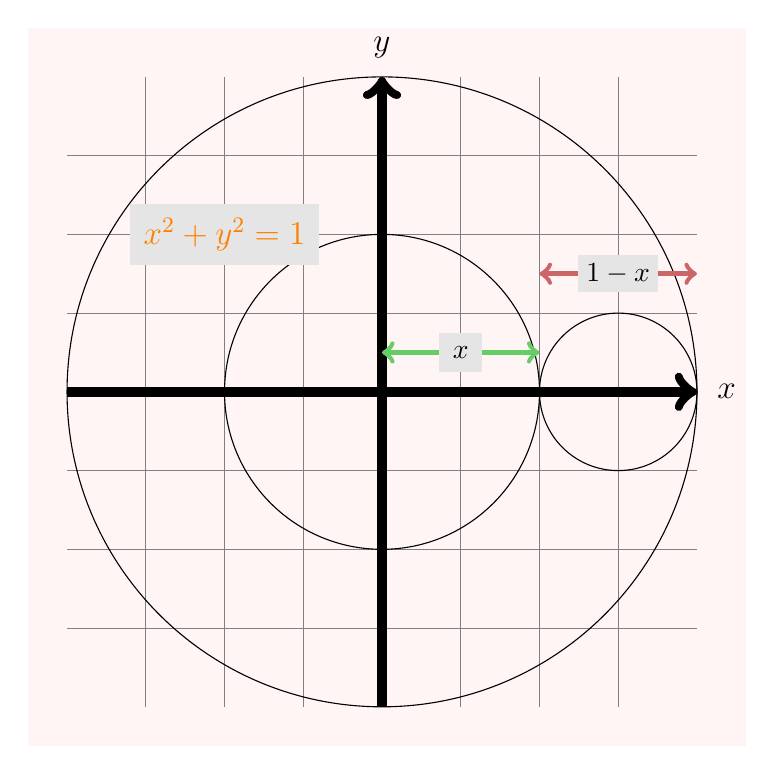
\begin{tikzpicture}

\fill[color=red!4!white] (-4.5,-4.5)--(-4.5,4.625)--(4.625,4.625)--(4.625,-4.5)--cycle;

\foreach \x in {-3,...,3}
	{
		\draw[color=black!50!white] (\x,-4)--(\x,4);
		\draw[color=black!50!white] (-4,\x)--(4,\x);
	}
	
\draw[->, line width=0.05in] (-4,0)--(4,0);
\draw[->, line width=0.05in] (0,-4)--(0,4);

\draw (0,0) circle (4);
\draw (0,0) circle (2);
\draw (3,0) circle (1);

\draw [<->, line width=0.025in, color=green!50!white!80!black] (0,0.5)--(2,0.5);

\node[fill=black!10!white, inner sep=5pt] at  (1,0.5) {\normalsize $x$} ; 

\draw [<->, line width=0.025in, color=red!50!white!80!black] (2,1.5)--(4,1.5);

\node[fill=black!10!white, inner sep=3pt] at  (3,1.5) {\normalsize $1-x$} ; 

\node[fill=black!10!white, inner sep=5pt] at (-2,2) {\color{orange}{\large $ {x^2 + y^2 = 1}$}};

\node at (4.375, 0) {\large $x$};

\node at (0, 4.375) {\large $y$};

\end{tikzpicture} \\ 
Let $a = \frac{1}{3}$.  I would like the image of these circles under the map:
$$ z \mapsto \frac{z - a}{\overline{a}z-1} $$


\newpage

\noindent \textbf{A} - the Easy Way \\ \\
This particular layout of circle is symmetric about the $x$ axis --- so we might\footnote{The small circle $|z-3|=\frac{1}{4}$ is moving in between $|z|=1$ and the image of $|z|=\frac{1}{2}$.  What happens (under inversion) if I rotate this figure? My question is what the image of the circle is under the map $z \mapsto  \frac{z - a}{\overline{a}z-1} $ and also $a = e^{i\theta} \frac{1}{3}$ and $\theta \in [0, 2\pi]$. } find an easier solution! \\ \\
The image of $x^2 + y^2 = \frac{1}{4}$ is itself a circle, symmetric about the $x$ axis.  
\begin{itemize}
\item $z = \frac{1}{2} \mapsto w = \frac{\frac{1}{2}-a}{\frac{1}{2}\overline{a}-1}$
and $z = -\frac{1}{2} \mapsto w = \frac{ - \frac{1}{2}-a}{-\frac{1}{2}\overline{a}-1}$

\item The center should be midway between them:
$$ \frac{1}{2} \left(
\frac{\frac{1}{2}-a}{\frac{1}{2}a-1}
+ 
\frac{-\frac{1}{2}-a}{-\frac{1}{2}a-1}
\right)
= \frac{3}{4} \times \frac{ a }{1 - \frac{1}{4} a^2} $$
\item and the radius should be half the difference 
$$ \frac{1}{2} \left(
\frac{\frac{1}{2}-a}{\frac{1}{2}a-1}
- 
\frac{-\frac{1}{2}-a}{-\frac{1}{2}a-1}
\right)
= \frac{1}{2} \times \frac{ - 1+ a^2 }{1 - \frac{1}{4}a^2} $$
\end{itemize}
\hrule \vspace{6pt}
The circle $(x - \frac{3}{4})^2 + y^2 = \frac{1}{4^2}$ has diameter $z = \frac{1}{2}$ and $z = 1$:
\begin{itemize}
\item $z = 1 \mapsto w = \frac{1-a}{a-1}= - 1$ and  easy computation:
$$ R = \frac{1}{2} \left(
\frac{\frac{1}{2}-a}{\frac{1}{2}a-1}
+
1 \right) \hspace{0.5in} C = \frac{1}{2} \left(
\frac{\frac{1}{2}-a}{\frac{1}{2}a-1}
- 1
\right) $$
\end{itemize}

\newpage

\noindent \textbf{B} - from Old Textbooks \\ \\
If $p$ and $q$ are inverse points on a Circle\footnote{This could be Ptolemy's Theorem since we are discussing power of a point.  I look at Titchmarsh's textbook on analysis and feel two ways: why are physicists skipping important steps even when they are very doable?  Why is the geometry limited to only one chapter?  Why not take a geometric approach to Hadamard's theorem or Lebesgue Theory?} that circle takes the form:
$$ \frac{|z- p|}{|z- q|} = k$$
and the map $z \mapsto f(z) = \frac{az+b}{cz+d}$ maps perfectly:
$$ \frac{|z- f(p)|}{|z- f(q)|} = k$$
This should feel awkard how to express the simple eq:
$$ |z| = \frac{1}{2}$$
which says that $0\leftrightarrow \infty$ are inverses.  Instead try:
$$ \frac{|z - \frac{1}{4} |}{|z - 1|} = \frac{1}{2}$$
and for the other circle $|z - \frac{3}{4}| = \frac{1}{2} $ a new formula:
$$  \frac{|z-\frac{5}{8}|}{|z-0|} = \frac{3}{8} $$
and hopefully our images agree.

\newpage

\noindent \textbf{C} - nnnooooooooo!!!! \\ \\
we just want a bit of detailed balanace making sure the algebra checks out. \\ \\
just because it is equation you think it is correct? 
\\ \\ LOL

\newpage

\noindent \textbf{D} - LOL

\newpage

\fontfamily{qag}\selectfont \fontsize{12}{10}\selectfont

\begin{thebibliography}{}

\item Curtis McMullen.  \textbf{Uniformly Diophantine Fixed Numbers in a Real Quadratic Field}

\item Jean Bourgain, Alex Kontorovich.
\textbf{Beyond Expansion II: Traces of Thin Semigroups} \texttt{arXiv:1310.7190v1}

\end{thebibliography}


\end{document}